    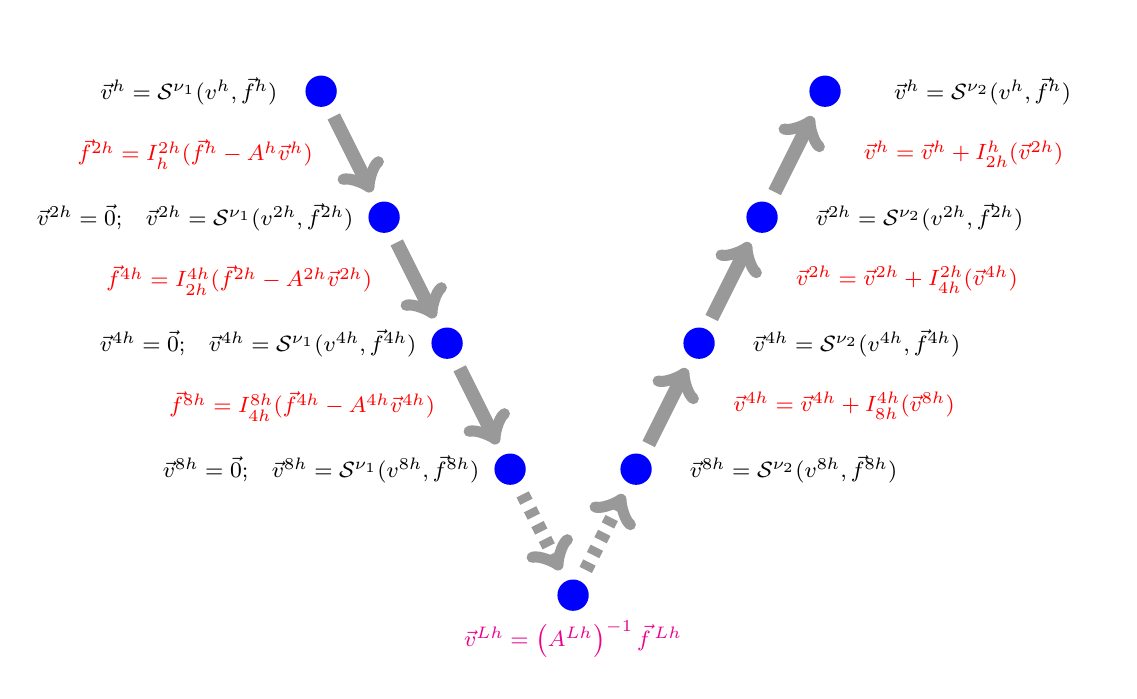
\begin{tikzpicture}[scale=0.8]
  \draw[white] (-8.5,9)--(8.5,9)--(8.5,-1.2)--(-8.5,-1.2)--cycle;
    \node[circle, fill=blue, inner sep=4pt,minimum size=2pt,line
    width=0pt] at (-4,8) {};

    \node at (-6.1,8) {\footnotesize $\vec{v}^h = 
      \mathcal{S}^{\nu_1}(v^h,\vec{f}^h)$};

    \draw[black!40,line width=5pt,->]
    (-3.8,7.6)--(-3.2,6.4);
    \node[red] at (-6.0,7.0) {\footnotesize $\vec{f}^{2h} = 
      I^{2h}_{h}(\vec{f}^h - A^h \vec{v}^h)$};
    \node[circle, fill=blue, inner sep=4pt,minimum size=2pt,line
    width=0pt] at (-3,6) {};

    \node at (-6,6) {\footnotesize $\vec{v}^{2h} = \vec{0}$;\quad $\vec{v}^{2h} = 
      \mathcal{S}^{\nu_1}(v^{2h},\vec{f}^{2h})$};

    \draw[black!40,line width=5pt,->]
    (-2.8,5.6)--(-2.2,4.4);
    \node[red] at (-5.3,5.0) {\footnotesize $\vec{f}^{4h} = 
      I^{4h}_{2h}(\vec{f}^{2h} - A^{2h} \vec{v}^{2h})$};
    \node[circle, fill=blue, inner sep=4pt,minimum size=2pt,line
    width=0pt] at (-2,4) {};

    \node at (-5,4) {\footnotesize $\vec{v}^{4h} = \vec{0}$;\quad $\vec{v}^{4h} = 
      \mathcal{S}^{\nu_1}(v^{4h},\vec{f}^{4h})$};

    \draw[black!40,line width=5pt,->]
    (-1.8,3.6)--(-1.2,2.4);
    \node[red] at (-4.3,3.0) {\footnotesize $\vec{f}^{8h} = 
      I^{8h}_{4h}(\vec{f}^{4h} - A^{4h} \vec{v}^{4h})$};
    \node[circle, fill=blue, inner sep=4pt,minimum size=2pt,line
    width=0pt] at (-1,2) {};

    \node at (-4,2) {\footnotesize $\vec{v}^{8h} = \vec{0}$;\quad $\vec{v}^{8h} = 
      \mathcal{S}^{\nu_1}(v^{8h},\vec{f}^{8h})$};

    \draw[black!40,line width=5pt,->,dashed]
    (-0.8,1.6)--(-0.2,0.4);
    \node[circle, fill=blue, inner sep=4pt,minimum size=2pt,line
    width=0pt] at (0,0) {};

    \node[magenta] at (0,-0.7) {\footnotesize $\vec{v}^{Lh} = 
      \left(A^{Lh}\right)^{-1} \vec{f}^{\,Lh}$};

    \draw[black!40,line width=5pt,->,dashed] (0.2,0.4)--(0.8,1.6);
    \node[circle, fill=blue, inner sep=4pt,minimum size=2pt,line
    width=0pt] at (1,2) {};

    \node at (3.5,2) {\footnotesize $\vec{v}^{8h} = 
      \mathcal{S}^{\nu_2}(v^{8h},\vec{f}^{8h})$};

    \draw[black!40,line width=5pt,->] (1.2,2.4)--(1.8,3.6);
    \node[red] at (4.3,3.0) {\footnotesize $\vec{v}^{4h} = 
      \vec{v}^{4h} + I^{4h}_{8h}(\vec{v}^{8h})$};
    \node[circle, fill=blue, inner sep=4pt,minimum size=2pt,line
    width=0pt] at (2,4) {};

    \node at (4.5,4) {\footnotesize $\vec{v}^{4h} = 
      \mathcal{S}^{\nu_2}(v^{4h},\vec{f}^{4h})$};

    \draw[black!40,line width=5pt,->] (2.2,4.4)--(2.8,5.6);
    \node[red] at (5.3,5.0) {\footnotesize $\vec{v}^{2h} = 
      \vec{v}^{2h} + I^{2h}_{4h}(\vec{v}^{4h})$};
    \node[circle, fill=blue, inner sep=4pt,minimum size=2pt,line
    width=0pt] at (3,6) {};

    \node at (5.5,6) {\footnotesize $\vec{v}^{2h} = 
      \mathcal{S}^{\nu_2}(v^{2h},\vec{f}^{2h})$};

    \draw[black!40,line width=5pt,->] (3.2,6.4)--(3.8,7.6);
    \node[red] at (6.2,7.0) {\footnotesize $\vec{v}^{h} = 
      \vec{v}^{h} + I^{h}_{2h}(\vec{v}^{2h})$};
    \node[circle, fill=blue, inner sep=4pt,minimum size=2pt,line
    width=0pt] at (4,8) {};

    \node at (6.5,8) {\footnotesize $\vec{v}^{h} = 
      \mathcal{S}^{\nu_2}(v^{h},\vec{f}^{h})$};

  \end{tikzpicture}
